\subsection{Señalización en fin de vía y transiciones}
    
	\label{sec:sig_border}
    
    % Autoridad > derecho limitado a una porcion
    % Claridad > autoridad no ambigua
    % Anticipacion > avisar con antelacion
    % Granularidad > rutas cortas y funcionales
    % Terminalidad > avisar fin de via
    % Infraestructura > avisar de infraestructura
    % No bloqueo > circulacion fluida

    Tal como se definió en la Sección \ref{sec:bufferstop}, las redes ferroviarias presentan tanto fines de vía absolutos (modelados en railML por la clase \textit{bufferStop}) como fines de vía relativos (modelados en railML por la clase \textit{lineBorder}). El RNA detecta estos elementos y generará el señalamiento correspondiente en base a los principios de señalamiento expuestos en la Sección \ref{sec:principios}.

    En el caso de las transiciones para fines de vía relativos, por el principio de infraestructura ($P_6$), es necesario que existan señales que indiquen que la formación pueda circular por la transición de una región ferroviaria a otra. Esta señal debe otorgar autoridad a la formación de forma unívoca, por el principio de claridad ($P_2$). Adicionalmente, esa señal debe situarse con suficiente antelación a la transición, por el principio de anticipación ($P_3$). Aplicando el principio de no bloqueo ($P_7$) regulamos la circulación entre dos regiones ferroviarias para que puedan circular sin demoras ni atascos. Finalmente, el principio de granularidad ($P_4$) y autoridad ($P_1$) nos pide que el derecho de uso de la infraestructura debe ser acotado, pero funcional. Es decir, la autoridad debe aplicarse en una sección con un mínimo de largo como para que tenga sentido. 

    En el Algoritmo \ref{alg:lineBorder} aplicamos todos estos principios al solicitar que la sección donde colocamos la señal tenga un parámetro de largo mínimo. Además, al ser una transición, las señales colocadas son todas de partida, para transitar de una región a la otra, de ser permitido, o detener la formación en la frontera entre ambas regiones, de encontrarse saturada la próxima región.
    
    \begin{algorithm}[H]
        \caption{Algoritmo de generación de señalamiento para Line borders.}\label{alg:lineBorder}
        \DontPrintSemicolon
        %\SetAlgoLined
        \SetNoFillComment
        \LinesNotNumbered 
        \For { netElement WITH LineBorder }
        {
            \If { netElement.Length $>$ FIXED\_LENGTH }
            {
                \If { NOT EXIST next netElement }
                {
                    [Signals] $\gets$ ADD departure signal $\gg\gg$\;
                }
                \If { NOT EXIST prev netElement }
                {
                    [Signals] $\gets$ ADD departure signal $\ll\ll$\;
                }
            }
        }
        \KwResult{[Signals]} 
    \end{algorithm}

    En el caso de los \textit{buffer stops}, por el principio de terminalidad ($P_5$) es necesaria una señal que indique a las formaciones que deben detenerse antes de llegar al final de la vía. Además, es necesaria una señal de partida en sentido contrario para que las formaciones reanuden su marcha en el otro sentido. Esto fue implementado en el Algoritmo \ref{alg:bufferStop}. La restricción de tamaño fue removida porque el final de vía y la formación deben ser protegidos sin importar el largo de la sección.
    
    \begin{algorithm}[H]
        \caption{Algoritmo de generación de señalamiento para Buffer stops.}\label{alg:bufferStop}
        \DontPrintSemicolon
        %\SetAlgoLined
        \SetNoFillComment
        \LinesNotNumbered 
        \For { netElement WITH BufferStops }
        {
            \If { NOT EXIST next netElement }
            {
                [Signals] $\gets$ ADD stop signal $\gg\gg$\;
                [Signals] $\gets$ ADD departure signal $\ll\ll$\;
            }
            \If { NOT EXIST prev netElement }
            {
                [Signals] $\gets$ ADD stop signal $\ll\ll$\;
                [Signals] $\gets$ ADD departure signal $\gg\gg$\;
            }
        }
        \KwResult{[Signals]} 
    \end{algorithm}
    
    Aplicando el Algoritmo \ref{alg:lineBorder} y el Algoritmo \ref{alg:bufferStop} a dos vías paralelas con finales de vías relativos (vía superior) y absolutos (vía inferior) obtenemos un señalamiento como el que se visualiza en la Figura \ref{fig:signal_border}.
    
    \begin{figure}[H]
        \centering
        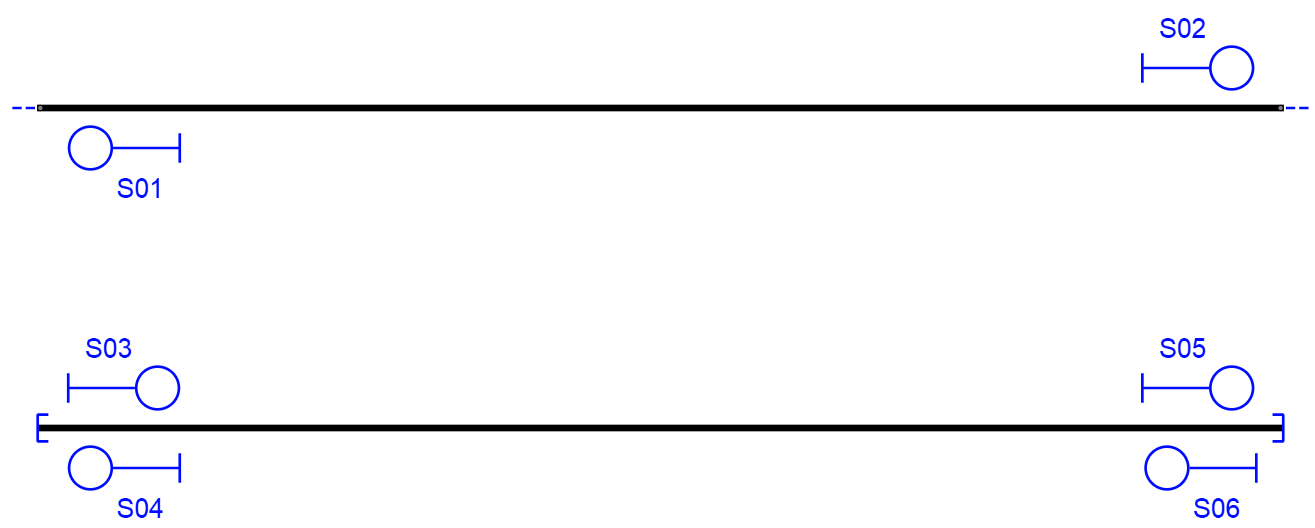
\includegraphics[width=1\textwidth]{Figuras/limites.PNG}
        \centering\caption{Señalamiento generado para finales de vía relativos y absolutos.}
        \label{fig:signal_border}
    \end{figure}
    
    El RNA detecta los \textit{line borders} en la vía superior y aplica el Algoritmo \ref{alg:lineBorder}, generando las señales de partida S01 para las formaciones que se mueven de derecha a izquierda y la señal de partida S02 para las formaciones que se mueven de izquierda a derecha, saliendo de la región mostrada en la Figura \ref{fig:signal_border}. Además, al detectar los \textit{buffer stops} en la vía inferior, el RNA aplica el Algoritmo \ref{alg:bufferStop}, generando cuatro nuevas señales. Las señales S04 y S05 son señales de parada para indicar a las formaciones que deben detenerse antes de colisionar con el final de la vía al transitar de derecha a izquierda o viceversa, respectivamente. Las señales S03 y S06 permiten a las formaciones reanudar su marcha en sentido contrario al que venían circulando, retomando su lugar en la red ferroviaria.